\documentclass[12pt]{amsart}
\usepackage[symbol]{footmisc}
\usepackage{float}
\usepackage{mathtools}
\usepackage{style_template}
\usepackage{hyperref}
\renewcommand*{\thefootnote}{\fnsymbol{footnote}}

% \newtheorem{theorem}{Theorem}
% \newtheorem{definition}{Definition}
\setlength\parindent{0pt}

\title{Young Mathematicians Conference Notes}
\author{David Yang}
\date{August 15th - 17th, 2023}

\begin{document}

\maketitle

\setcounter{section}{-1}
\section{Overview}

These are my collection of notes from my experience at the Young Mathematicians Conference, held from August 15th to 17th, 2023 at Ohio State University. 
I take any responsibility for typos/incorrect definitions -- I was only able to write down and follow part of each presentation. Feel free to contact each of the speakers for any questions and to look over the official YMC Abstracts (some of the notes here are from them), which you can find \href{https://ymc.osu.edu/sites/default/files/2023-08/ymc_2023-2.pdf}{here}. \\

These notes serve as a catalogue for my academic conference experience -- feel free to read more about my personal (general) conference experience \href{https://github.com/dyang5/CirclePackingsResearch/blob/main/Conferences/writeups/YMC_Writeup.md}{here}!

\vspace{2cm}
\section{Day 1: August 15th}

\vspace{0.25cm}


\subsection{The Failed Zero Forcing Number of a Graph}

\textit{}
\vspace{0.25cm}

\textit{Presented by Chirag Kaudan and Rachel Taylor.}

\begin{definition}[Forcing Rule]
Let each vertex of a graph represent a person. Each person either knows or does not know a secret -- if they do, their corresponding vertex is colored. \\

If all a person's friends except one friend knows the secret, then the secret is told to that friend as well.\end{definition}

\begin{definition}[Zero Forcing Number]
The zero forcing number of $G$, $Z(G)$, is the smallest cardinality of any set $S$ of vertices on which repeated applications of the forcing rule
results in all vertices joining $S$.
\end{definition}

\begin{definition}[Failed Zero Forcing Number]
The failed zero forcing number of $G$, $F(G)$, is the maximum
cardinality of any set of vertices on which repeated applications of the forcing rule will never result in all vertices joining the set.\end{definition}

\begin{result*}
Using the theory of \textit{modules} (a set of vertices such that every vertex in the module has the same neighorhood exclusing vertices in the module) in zero forcing graphs and a computer algorithm, they were able to show that
there are $15$ graphs with $F(G) = 2$ and $68$ graphs with $F(G) = 3$. 
\end{result*}

\vspace{2cm}

\subsection{Properties of Families of Graphs with Forbidden Induced Subgraphs}

\textit{}
\vspace{0.25cm}

\textit{Presented by Christian Pippin.}

\begin{definition}[Induced Subgraphs]
$H$ is an \textbf{induced subgraph} of $G$ if the vertex set of $H$ is a subset of the vertex set of $G$ and for all $(u, v) \in E^{H}$, $(u, v) \in E^G.$
\end{definition}

There is a relation between indivisibility and the lex product. \\

\begin{lemma*}
If a family of graphs is closed under the lex product, the class is indivisible.
\end{lemma*}

\begin{theorem*}
For all $n$, $\mathrm{Forb}(P_n)$ is indivisible. \\

$\mathrm{Forb}(C_n)$ is indivisible for all $n \geq 5.$
\end{theorem*}

\vspace{2cm}

\subsection{Generalized Stick Fragmentation and Benford's Law}

\textit{}
\vspace{0.25cm}

\textit{Presented by Xinyu Fang and Maxwell Sun.}

\begin{theorem*}[Benford's Law]
In base $B$, the probability of observing a value with first digit $d$ is \[ \log_B\left(\frac{d+1}{d}\right).\]

If this property holds, a dataset is said to exhibit \textbf{weak Benford behavior}; if, moreover, the logarithms of the values modulo 1 are equidistributed, then the set exhibits \textbf{strong Benford behavior}. 
\end{theorem*}

\begin{definition}[Significand and Mentissa]
The \textbf{significand} of $x$ base $B$ is $S_B(x) \in [1, B)$ such that $x = S_B(x) \cdot B^k$ for some $k$. \\

The \textbf{mantissa} is the analogue but for fractional pieces.
\end{definition}

\vspace{0.5cm}

To setup the problem, consider a stick breaking model where you begin with a stick of length $\ell$. At each step, the stick is broken into smaller segments and this process continues until some termination condition is reached. The problem the authors studied is known as a \textit{Discrete Breaking Problem with a Stopping Set}: if the stick length falls into the given stopping set, it is considered ``dead" and should not be broken further. \\

\begin{result*}
The authors give some results on when a given set of end lengths is Strong Benford (for which types of stopping sets). \\

In particular, they conjecture that if you break each stick into $k$ parts and stop at $(k-1) \cdot \frac{n}{k}$ residue classes modulo $n$ where $k \mid n$, then the results are Strong Benford.
\end{result*}

\vspace{2cm}

\subsection{Geometry of the Numerical and Berezin Range}

\textit{}
\vspace{0.25cm}

\textit{Presented by Edwin Xie and Caroline Norman.}

\begin{definition}[Numerical Range]
The \textbf{numerical range} $f$ of a bounded linear operator $T$ on a complex Hilbert space $H$ is defined as
\[ W(T) = \{\langle Tf, f \rangle : ||f|| = 1.\} \]

Properties of the numerical range include unitary invariance, shift and scale, and that it satisfies the Topelitz-Hausdorff property.
\end{definition}

\begin{definition}[Berezin Range]
On the Hardy-Hilbert space $H^2(\mathbb{D})$ of the open unit disk $\mathbb{D}$, the \textbf{Berezin range} is defined as 
\[B(T) = \{ \langle T\hat{k}_p, \hat{k}_p \rangle : p \in \mathbb{D}\}\]
where $\hat{k}_p$ is the normalized reproducing kernel.

\end{definition}
\begin{result*}
The authors work with the Berezin Range on a Hardy Space and prove some results about the Berezin Range.
\end{result*}

\vspace{2cm}

\newpage

\subsection{The VC Dimension of Semi-Algebraic Sets}

\textit{}
\vspace{0.25cm}

\textit{Presented by Kayta Gheorghian.}

\begin{definition}[VC Dimension]
Let $X$ be a set and $F$ a family of subsets of $X$. Then for any subset
$A \subseteq X$, we say that $F$ shatters $A$ if for each $A' \subseteq A$ there exists $F' \in F$ such that $F' \cap A = A'.$ \\

The \textbf{Vapnik-Chervonenkis (VC) dimension} of $X$ with respect to $F$ is
\[ \max_{A \subseteq F} |A| : F \text{ shatters } A.\]
\end{definition}

\begin{definition}[Heisenberg Group]
The Heisenberg Group is defined as the following group of $3 \times 3$ upper triangular matrices: \[\mathcal{H}(\mathbb{Z}) = \left \{\begin{bmatrix} 1 & a & b \\ 0 & 1 & c \\ 0 & 0 & 1\end{bmatrix}, \, a, b, c \in \mathbb{Z} \right\}.\]
\end{definition}

\begin{result*}
In attempting to find the VC Dimension of the Heisenberg group, they studied a related problem -- the VC Dimension of different quadrilaterals in $\mathbb{R}^2$.
\end{result*}

\newpage

\subsection{The Collatz Conjecture over the Gaussian Integers}

\textit{Plenary Lecture.}
\vspace{0.25cm}

\textit{Presented by Professor Alejandra Alvarado (Eastern Illinois University).\footnote{Her presentation was created after a 2017 REU project, so certain details may be older results.}}

\begin{definition}[Collatz Conjecture]
Define the function \[ f(n) = \begin{cases}\frac{n}{2} & \text{if n is even} \\ 3n + 1 & \text{if n is odd} \end{cases}.\]
Form a sequence by repeatedly applying this function. \\

\textbf{The Collatz Conjecture} states that the hailstone sequence/trajectory will eventually reach $1$, regardless of the starting positive integer.
\end{definition}

\vspace{0.25cm}

A heuristic probabilistic argument by Crandall in 1978 gives an argument for non-divergence (each odd number is on average $\frac{3}{4}$ of the previous odd number), but the question of whether the sequence always reaches $1$ remains unsolved (though apparently the conjecture has been shown to hold up to $5 \times 2^{68}$ computationally). \\

Extensions of the Collatz Conjecture may arise when the collatz function is generalized or the question is extended to other rings. For example, the speaker proposes extending the Collatz Conjecture to the Gaussian and Eisenstein Integers.

\begin{definition}[Gaussian Integers]
The \textbf{Gaussian Integers} are the set $\mathbb{Z}[i] : \{ a + bi \mid a, b \in \mathbb{Z} \}.$ \\
    
Useful facts include that if $p \equiv 3 \pmod 4$, then $p$ is a Gaussian Prime. If $p \equiv 1 \pmod 4$ where $p = (a+bi)(a-bi)$, then $a+bi$ is a Gaussian prime.
\end{definition}

\begin{definition}[Eisenstein Integers]
The \textbf{Eisenstein Integers} are the set $\mathbb{Z}[\omega] : \{ a + b\omega \mid \omega^2 + \omega + 1 = 0 \}.$ \\
\end{definition}

\begin{result*}
The speaker discusses the construction of a spiral ordering of Gaussian integers in the first quadrant, and discusses a Gaussian Collatz Mapping, as well as the trajectories of various Gaussian Integers under this mapping. \\

Afterwards, she also discusses similar approaches/results for the Eisenstein Integers.
\end{result*}

\newpage

\section{Day 2: August 16th}

\subsection{Practical Uses of Complex Analysis}

\textit{Plenary Lecture.}
\vspace{0.25cm}

\textit{Presented by Professor Loredana Lanzani of Syracuse University and University of Bologna.}

\begin{definition}[Conformal Maps]
\textbf{Conformal Maps} are maps $f: \mathbb{C} \rightarrow \mathbb{C}$ that
\begin{itemize}
    \item on a small scale, preserve the shape of objects (i.e. angles between intersecting curves are preserved) 
    \item on a large scale, may greatly distort shapes
\end{itemize}

\end{definition}

\vspace{0.25cm}
Examples of conformal maps include translations, rotations about a point, dilation, inversion, the \textbf{Joukowski Map} $f(z) = z + \frac{1}{z}$, as well as complex powers $f(z) = z^\alpha, \, \alpha \in \mathbb{C}.$ \\

Another example is the classic example of \textbf{stereographic projection} (which projects points on a spheroid directly to the plane). As a historical aside, the speaker talked about a painting by Ruben in 1613 depicting Ptomeley: \\

\begin{center}
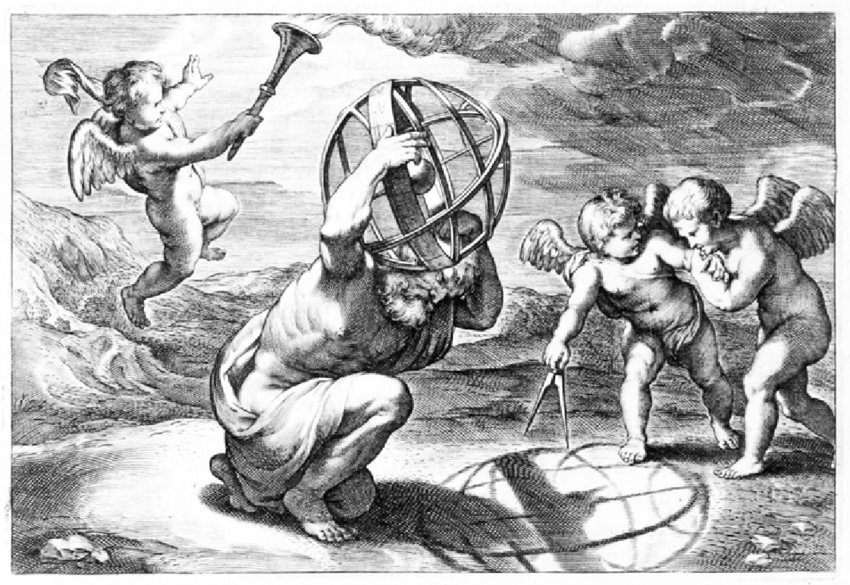
\includegraphics[scale = 0.35]{note_imgs/ruben_ptolemy.png}
\end{center}

In particular, in the center of Ruben's universe the Earth or the Sun? It turns out that according to the size of the angles (the power of conformal maps is on full display), it is the Earth. \\ 

Other applications of conformal maps include cartography, in the Droste Effect in art, aircraft-wing design, and in morphology. \\

In \textbf{cartography}, the goal is to design a (flat) map of the world that sailors can use for exploration. 
Consequently, the stereographic projection map discussed early has the effect of large scale area distortion (for example, Greenland and Africa are missized relative to each other). However, the stereographic projection does allow for a map with no cuts and gives good accuracy on a small scale. 
On the other hand, a method known as Localized Stereographic Projection may work better. This projection is a type of polar stereographic projection used for navigation in polar regions -- the localization of this map is key, which correlates with the property of conformal maps. \\

Conformal maps also show up in art. 

\begin{definition}[Droste Effect]
The \textbf{Droste Effect} is a repeating visual effect that occurs when an image contains a copy of that (same) image, which in turn contains the copy of that ... and so on and so forth.
\end{definition}

This effect is named after the following picture, of Droste cocoa powder, where you can see that the nurse is carrying a serving tray with a cup of hot chocolate and a box with the same image. 

\begin{center}
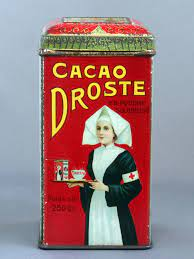
\includegraphics[scale = 0.75]{note_imgs/droste_effect.jpeg}
\end{center}

It turns out that Droste pictures can be obtained by applying the conformal map \[f(z) = z^\alpha \text{ with } \alpha = 1 - i \frac{1}{2\pi} \log(s_o) \] where $s_o$ represents the scaling factor of a Droste image (the larger the scaling factor, the harder to see each iteration -- in the above photo, the scaling factor is around $6.5$). \\

Another famous painting that makes use of the Droste effect (scaling factor $\sim 256$) is M. C. Esher's \textit{Print Gallery} from 1956:

\begin{center}
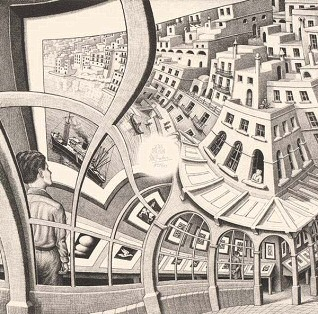
\includegraphics[scale = 0.8]{note_imgs/escher_print_gallery.jpg}
\end{center}

You may notice that in the center of the image, there is a blank space. Mathematicians have tried to use the Droste effect and conformal maps to study/determine the art that could possibly fill this hole. The speaker specifically mentions \textit{Complexities of Art} by Kay Horak of Smith College as a resource to study (I could not find this online); 
there are many others online that may be worth reading as well. \\

In aircraft wing design, the goal is to design an airplane wing that produces force/life strong enough to keep it in the air. One solution is to apply a Joukowski map (a type of conformal map) to a circle -- this will get airfoil and will allow you to study the airflow surrounding it. \\

D'Arcy Wentworth Thompson (1860-1948)'s ``On Growth and Form'' explored the extent to which relationships among different species of animals can be described as conformal transformations. Homologous pairs of animals must ``preserve a given number of landmark points'' (at least 7). However, this means that there cannot be a conformal mapping between 
these pairs since conformal mappings can only guarantee at most 3 landmark points. Thus, \textbf{quasi-conformal mappings} are introduced. This allows for (controlled) angle deformation and allows for lots of homologous landmark points. \\

The final example of conformal mappings was in the study of the time evolution of \textit{Monstera Delicosa} (Swiss cheese plant) and modeling its fenestration phenoma. \\

\newpage

\subsection{A Structure Theorem on Doubling Measures as Arbitrary Bases}

\textit{}

\vspace{0.25cm}
\textit{Presented by Zoe Markman and Teresa Pollard.} \\

\begin{definition}[Doubling Measure]
A \textbf{doubling measure} is a measure $\mu$ satisfying \[ \frac{1}{C} \leq \frac{\mu(I)}{\mu{J}} \leq C \]
where $I$ and $J$ are adjacent intervals of the same length.
\end{definition}

\begin{definition}[p-adic]
A \textbf{p-adic interval} is $[\frac{k}{p^n}, \frac{k+1}{p^n}]$ forany $k, n \in \mathbb{Z}$ and some prime $p$. \\

A \textbf{p-adic doubling measure} satisfies the above property of a doubling measure where $I, J$ are any two children of a given p-adic interval.
\end{definition}

\begin{result*}
The speakers proved some structure theorems of these doubling measures as part of their research project: \\

``A 2022 paper by Anderson and Hu constructs a measure which is $p$ and $q$-adic doubling for distinct primes $p, q$ but not
doubling overall. The construction of this measure relies heavily on an established number
theory framework, which allows for the selection of an infinite family of $q$-adic intervals ``close
enough" to $p$-adic intervals such that the Lebesgue measure can be reweighted on these $q$-adic
intervals in a way that preserves $p$ and $q$-adic doubling, while breaking doubling overall. We
generalize the number theory involved in this construction to create a measure that is $n$-adic
doubling and $m_1, \dots, m_k$-adic doubling for any $n \in \mathbb{N} > 1$, such that each mi
is a multiple of some $c$ coprime to $n$. We then provide a further generalization of the analysis used by Anderson
and Hu to construct a measure that is $n$-adic doubling for every $n \in \mathbb{N} > 1$ but not doubling
overall."
\end{result*}

\newpage

\subsection{Binomial Sets under $\mathbb{Z}$-Linear Forms}

\textit{(Presentation Title: Phase Transitions and Point Process Limits for Generalized Sumsets of Binomial Random Sets)}

\textit{}

\vspace{0.25cm}
\textit{Presented by Ryan Jeong.}

\begin{definition}[MSTD]
Consider a set $A \subseteq \{0, 1, \dots, N\}.$ \\

The \textbf{sum and difference sets} are \[ A + A \coloneqq \{a_1 + a_2: a_1, a_2 \in A \} \text { and } A - A \coloneqq \{a_1 - a_2 : a_1, a_2 \in A \}.\] 

A set is \textbf{MSTD} (More Sum Than Differences Set) if $|A+A| > |A-A|.$
\end{definition}

\begin{result*}
    The speaker works on generalized sumsets (of $s$ sums and $d$ differences), proving some results for these sumsets. A key component of their approach is Stein's Method, which they also explain.
\end{result*}

\vspace{2cm}

\subsection{Generalizations of the Erdos-Ginzburg-Ziv Theorem via Topology}

\textit{}

\vspace{0.25cm}
\textit{Presented by Jacob Lehmann Duke, Hannah Park-Kaufmann, and Meenakshi McNamara.}

\begin{theorem*}[Erdos-Ginzburg-Ziv]
Any sequence of $2n - 1$ numbers in $\mathbb{Z}/n$ has a subsequence of length $n$ that sums to zero
\end{theorem*}

\begin{result*}
    We develop a novel topological approach, based on the non-existence of continuous maps that commute with certain
    symmetries, to prove that the permutations whose difference gives the zero-sum subsequence
    may be strongly restricted. \\

    They prove these results using a number of different topological approaches, including chessboard complexes, probability measures, and more.
\end{result*}

\newpage

\subsection{On the Size and Complexity of Scrambles}

\textit{}

\vspace{0.25cm}
\textit{Presented by Steven DiSilvio and Krish Singal.}

\begin{definition}[Chip-Firing Graph]
Let $G$ be a connected, loopless multigraph with vertices $V = \{1, 2, \dots, n\}.$ \\

A \textbf{chip-firing game} is played on such a graph by placing an integer number of chips on each node of the graph, and then moving them around according to chip-firing moves, where one node donates chips to its neighbors, one along each edge. 
(If a vertex has a negative value, it means they are ``in debt'').\end{definition}

\begin{definition}[Relevant Definitions]
The \textbf{gonality} of a graph $G$ $\mathrm{gon}(G)$ is the smallest $k$ such that there exists a placement of $k$ chips on $G$ guaranteed to eliminate a $-1$ debt placed anywhere on $V(G)$ without introducing debt elsewhere. \\

A \textbf{scramble} $S$ is a collection of connected subgraphs of $G$ (called eggs). The \textbf{hitting number} is the minimum number of vertices needed to hit each egg in a scramble.
\end{definition}


\begin{result*}
To study these chip-firing games, the speakers study the scramble numbers of graphs, which help give lower bounds for gonality as per Harp et. al. (2022), which states that \[ \mathrm{Sc}(G) \leq \mathrm{gon}(G)\] for all graphs G.
\end{result*}

\vspace{2cm}

\subsection{Stiffness matrices and d-dimensional algebraic connectivity}

\textit{}

\vspace{0.25cm}
\textit{Presented by Yunseong Jung.} \\

I was not able to take notes for this presentation -- see YMC abstract page for more information.

\newpage

\section{Day 3: August 17th}

\subsection{Topology Meets Physics: Scissors Congruences and TQFT}

\textit{Plenary Lecture.}
\vspace{0.25cm}

\textit{Presented by Professor Carmen Rovi (Loyola University).} \\

The talk relates Topology (Manifolds/Scissor Congruences) with Physics (TQFT). \\

\begin{definition}[Scissors Congruence]
Two shapes are \textbf{scissors congruent} if you can chop/cut one shape into pieces and rearrange those pieces along their boundaries to form the other shape. \\

Scissors congruent and cut and paste equivalent are equivalent.
\end{definition}

\textit{Note:} area is invariant under this cut and paste operation on polygons; however, this does not generalize to 3D shapes and volume.

\begin{definition}[Manifold]
A \textbf{$n$-dimension manifold} is a space that locally resembles $\mathbb{R}^n$. (1D: circle, 2D: sphere, torus) \\

A \textbf{$n$-dimension manifold with boundary} is a space that resembles
\begin{itemize}
    \item $\mathbb{R}^n$ on each neighborhood of all its interior points
    \item $\mathbb{R}^+ \times \mathbb{R}^{n-1}$ on each neighborhood of points on the boundary.
\end{itemize}
\end{definition}

\begin{definition}[Homeomorphism]
Two spaces are \textbf{homeomorphic} if one can be distorted to make the other.
\end{definition}

Topology uses algebraic invariants (e.g. the Euler characteristic) to analyze properties of manifolds and answer classification problems.

\begin{definition}[Cobordism]
Two $n$-dimensional manifolds $M$ and $M'$ are \textbf{cobordant} if there exists an $(n+1)$ dimensional manifold $W$ such that $M$ and $M'$ form the boundary of $W$. \\

Cobordism forms an equivalence relation on manifolds.
\end{definition}

\begin{definition}[TQFT]
A $n$-dimensional \textbf{topological quantum field theory} (TQFT) is a functor that assigns
\begin{itemize}
    \item a finite dimension vector space to each $(n-1)$ dimensional manifold
    \item a linear map to a bordism between them
\end{itemize}
\end{definition}

\newpage

\subsection{Circle Packings from Tilings of the Plane}

\textit{}

\vspace{0.25cm}

\textit{Presented by David Yang (me).} \\

Feel free to check out my presentation \href{https://github.com/dyang5/CirclePackingsResearch/blob/main/presentations/YMC_Presentation.pdf}{here}, or read about my conference experience \href{https://github.com/dyang5/CirclePackingsResearch/blob/main/Conferences/writeups/YMC_Writeup.md}{here}! I am happy to answer any questions about my project :)

\vspace{2cm}

\subsection{Dehn Invariant Zero Tetrahedra} 

\textit{}

\vspace{0.25cm}

\textit{Presented by Anas Chentouf.}

To answer the question of when two polyhedra are scissors congruent, one can use the Dehn Invariant.
\begin{definition}[Dehn Invariant]
The \textbf{Dehn Invariant} is a value used to determine whether one polyhedron can be cut into pieces and reassembled into another, and whether a polyhedron or its dissections can tile space.
\end{definition}

\begin{theorem*}[Scissors Congruence and Dehn Invariant]
If two polyhedra are scissors congruent, their Dehn Invariant are equal. \\

If two polyhedra have the same volume and the same Dehn invariant, they are scissors congruent.
\end{theorem*}

\begin{theorem*}[Debrunner, 1980]
If a tetrahedron tiles space, it has Dehn invariant $0$ (the converse does not hold).
\end{theorem*}

Thus, instead of studying tiling tetrahedra (since the only way to prove a tetrahedron tiles is to exhibit an explicit tiling), one can classify Dehn Invariant Tetrahedra.

\begin{result*}
From the speaker's YMC abstract:
``We contribute previously unknown families of tetrahedra of Dehn
invariant zero (DI0), as well as some sporadic tetrahedra. We also show that there are finitely
many Dehn invariant zero tetrahedra whose dihedral angles have a five-dimensional span over
$\mathbb{Q}$, a first step towards classifying all Dehn invariant zero tetrahedra. We also exhibit a Dehn
invariant zero tetrahedron that does not tile, thereby answering a previously open question."
\end{result*}

\newpage

\subsection{Distance Graph Embeddings over Finite Fields} 

\textit{}

\vspace{0.25cm}

\textit{Presented by Xinyu Fang and Maxwell Sun.}

\begin{definition}
Let $q$ be an odd prime power. For $x, y \in \mathbb{F}_q^d$, define \[ || x-y|| = \sum\limits_{i=1}^d (x_i - y_i)^2.\]

For $E \subseteq \mathbb{F}_q^d$, let $\Delta(E) = \{ || x-y||: \, x, y \in E\}.$
\end{definition}

The \textbf{Erdos distance problem} asks how small can $|\Delta(E)|$ be as $E$ gets bigger.

\begin{result*}The speakers discuss their results for various distance problems, on embedding new families of distance graphs which are formed from certain basic
configurations: ``These include the k-fold Holder extension of 3-chains and chains of equilateral
triangles, which have not been studied previously. Our results in these cases make significant
improvements on the bounds given by the general case by exploiting symmetries within the
graphs and sophisticated inductive arguments. Moreover, in order to lower bound nondegenerate embeddings, we make clever counting arguments of degeneracies that use the geometry
of finite field vector spaces."
\end{result*}
\end{document}
